\chapter{Implementación}

Con el fin de experimentar con los algoritmos de planificación de flujos de trabajo, se implementaron algunos algoritmos descritos en este trabajo. Los algoritmos fueron implementados en Java.

Se implemetaron los algoritmos Miope, MinMin y MaxMin. El algoritmo Miope es un algoritmo voraz que sólo busca el recurso que pueda ejecutar la tarea lo más pronto posible. Los algoritmos MinMin y MaxMin buscan recursos que puedan minimizar tanto la duración de la tarea como el tiempo en el que inician las tareas. Luego, en el caso de MaxMin, se busca la tareas que sean más tardada de ejecutar ó, en el caso de MinMin, se busca la tarea que tarde menos en ejecutarse.

Ahora, se hicieron dos supocisiones para simplificar la implementación:

\begin{enumerate}
\item Los recursos pueden ejecutar todas las tareas.
\item Para el caso de los algoritmos MaxMin y MinMin, el tiempo de disponibilidad de transferencia de archivos es el tiempo en que las tareas inmediatamente precedentes han sido ejecutadas, asumiendo que la transferencia de datos entre nodos es instantánea.
\item Una tarea es considerada lista para planificarse si todos sus predecesores inmediatos han sido planificados.
\item Los recursos ejecutan una sola tarea a la vez.
\end{enumerate}

\section{Descripción del código}
El diseño de las clases y objetos se hizo de tal modo que los elementos más comunes de los algoritmos fueran representados en una clase. Así, describiremos primero las clases \texttt{Task}, \texttt{Resource} y \texttt{Schedule}, para luego describir la clase \texttt{Workflow} y las clases que implementan los algoritmos: \texttt{Myopic}, \texttt{MinMin} y \texttt{MaxMin}. En la figura \ref{fig:uml_class} se puede apreciar el diagrama de clases UML de las clases que modelan los elementos del problema de planificación de flujos de trabajo.

\begin{figure}
\label{fig:uml_class}
\begin{center}
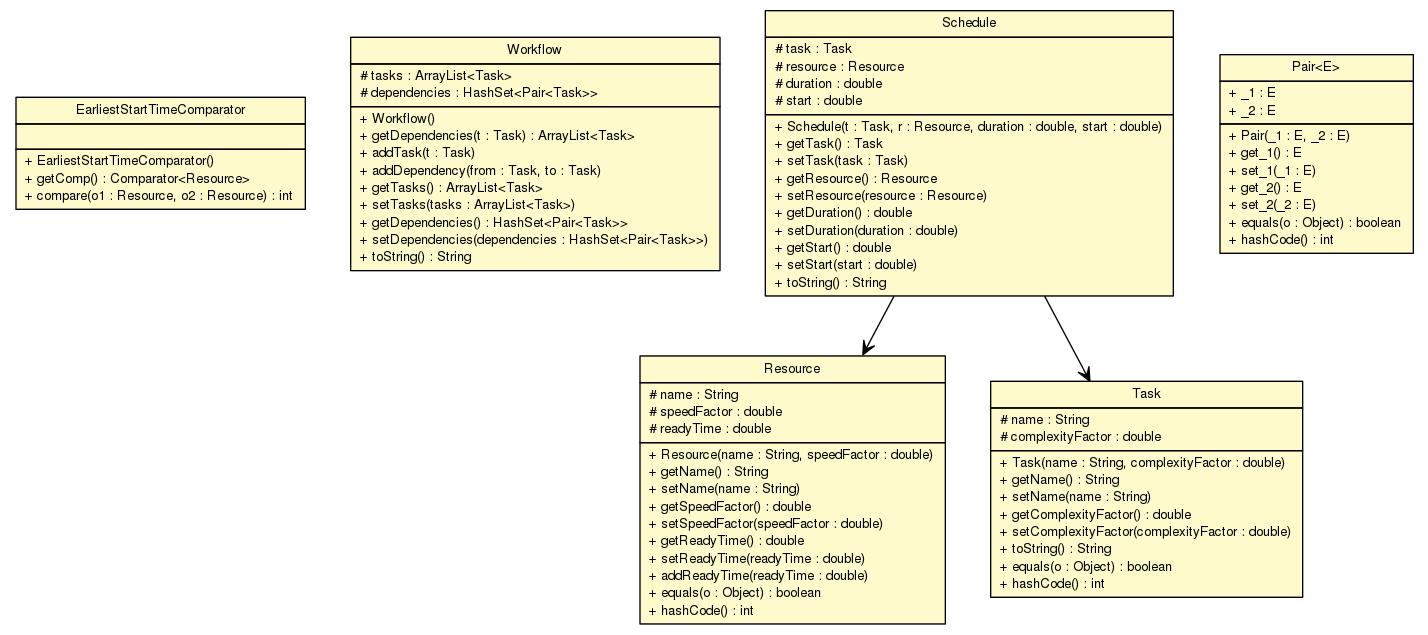
\includegraphics[width=1.0\textwidth]{imagenes/uml_class}
\end{center}
\caption{Diagrama de clases UML de las clases principales.}
\end{figure}

\subsection{Clase \texttt{Task}}
La clase \texttt{Task} representa una tarea que forma parte de un flujo de trabajo. Cada tarea tiene un nombre que debe ser único en el flujo de trabajo del que forma parte. También, la tarea contiene un factor de complejidad, que es un número que representa qué tan complicado es ejecutar esta tarea. La idea básica es que a mayor factor de complejidad, mayor es el tiempo requerido para ejecutar la tarea o un recurso más rápido es necesario para ejecutar la tarea. 

\subsection{Clase \texttt{Resource}}
En esta clase se representa a un recurso que puede ejecutar tareas de un flujo de trabajo. De forma similar a la clase \texttt{Task}, un recurso tiene un nombre --que no es necesario que sea único-- y un factor de velocidad que indica la rapidez con la que dicho recurso puede ejecutar una tarea.

\subsection{Clase \texttt{Schedule}}
Representa una planificación de una tarea en un recurso. Cada objeto de esta clase guarda la tarea y el recurso que fueron asignados, el tiempo en que se empezará a ejecutar la tarea y el tiempo estimado de ejecución de la tarea en el recurso.

\subsection{Clase \texttt{Workflow}}
La clase \texttt{Workflow} representa un flujo de trabajo, compuesto de tareas y las relaciones de precedencia entre tareas. Cabe aclarar que no se permiten que existan tareas con el mismo nombre y también se verifican que las relaciones de precedencia entre tareas formen un grafo dirigido acícilico.

\section{Código de los algoritmos}
En esta sección, detallaremos las decisiones de diseño que fueron necesarias para implementar los algoritmos.

\subsection{Algoritmo Miope}
Como se vió en el capítulo \ref{chap:scheduling_algorithms} y en la sección \ref{alg:myopic} del Apéndice, el algoritmo Miope asigna tareas a recursos de tal modo que se empiecen a ejecutar lo más pronto posible. Aunque la idea básica resulte fácil de entender, hay algunas cuestiones que deben ser resueltas para implementar este algoritmo.

Primero, hay que tomar en cuenta cómo obtener tareas que estén listas para planificarse. Para ello, se planifican sólo aquellas tareas cuyos predecesores inmediatos o padres han sido planificados. Cabe aclarar que se entiende que una tarea está planificada si ésta ya está asignada a un recurso, por lo que no se permite que una tarea sea asignada a varios recursos.
De esta forma para generar la lista de tareas a planificar, se seleccionan aquellas tareas que no han sido planificadas y cuyos padres ya han sido planificados. Este último requerimiento asegura que se respeten las dependencias entre tareas a la hora de planificar. está implementado en el método estático \texttt{Utils.checkParents()}. Por otro lado, para verificar si una tarea está planificada, se excluyen de la lista de tareas a planificar aquellas tareas ya planificadas.

En la figura \ref{code:myopic} está el código en Java del algoritmo miope, utilizando las clases antes descritas. Cabe notar que para conocer cuál es el recurso más disponible, se mantiene una cola de prioridad de los recursos con el tiempo de disponibilidad más pronto.

\begin{figure}
\label{code:myopic}
\begin{lstlisting}[language=java]
List<Schedule> schedule(Workflow w, List<Resource> resourceList) {
  Utils.checkScheduleParams(w, resourceList);
  //lista de tareas no calendarizadas
  ArrayList<Task> readyTasks = new ArrayList<Task>(w.getTasks());
  ArrayList<Task> schedTasks = new ArrayList<Task>();
  ArrayList<Schedule> schedules = new ArrayList<Schedule>();
  //heap para mantener a los recursos mas pronto disponibles
  PriorityQueue<Resource> R = new PriorityQueue<Resource>(resourceList.size(), EarliestStartTimeComparator.getComp());
  R.addAll(resourceList);
  Task t; Resource r;
  while(!readyTasks.isEmpty()) {
    Iterator<Task> it = readyTasks.iterator();
    if(it.hasNext()) {
      t = it.next();
      if(Utils.checkParents(t, schedTasks, w)) {
        r = R.peek();
        double d = t.getComplexityFactor() / r.getSpeedFactor();
        double st = Math.max(r.getReadyTime(), Utils.parentsReadyTime(t, schedules, w));
        Schedule s = new Schedule(t, r, d, st);
        readyTasks.remove(t);
        schedTasks.add(t);
        r.addReadyTime(d);
        //Actualizamos heap
        R = new PriorityQueue<Resource>(resourceList.size(), EarliestStartTimeComparator.getComp());
        R.addAll(resourceList);
        schedules.add(s);
      }
    }
  }
  return schedules;
}
\end{lstlisting}
\caption{Código en Java del algoritmo Miope}
\end{figure}

\subsection{Algoritmo MaxMin y MinMin}
Para los algoritmos MaxMin y MinMin se utilizaron varias métodos desarrollados para el algoritmo miope. Por ejemplo, el método \texttt{Utils.parentsReadyTime()} utilizado para obtener cuándo terminaran de ejecutarse todas las tareas que son predecesores inmediados de una tarea en flujo de trabajo dada una calendarización. Como se vio en la sección \ref{alg:def_maxmin} del Apéndice, hay algunas definiciones que son comunes para ambos algoritmos. En la figura \ref{code:xmin_defs} están codificadas dichas definiciones.


\begin{figure}
\label{code:xmin_defs}
\begin{lstlisting}[language=java]
/** Estimated Execution Time */
private static double EET(Task t, Resource r) {
  return t.getComplexityFactor() / r.getSpeedFactor();
}

/** Estimated Availability Time */
private static double EAT(Task t, Resource r) {
  return r.getReadyTime();
}

/** File Available Time */
private static double FAT(Task t, Resource r, Workflow w, List<Schedule> partialSchedule) {
  //le vamos a dar una "semantica" diferente
  //tomamos el tiempo de los padres como el tiempo de archivos listo
  return Math.max(r.getReadyTime(), Utils.parentsReadyTime(t, partialSchedule, w));
}

/** Estimated Completion Time */
private static double ECT(Task t, Resource r, Workflow w, List<Schedule> partialSchedule) {
  return EET(t, r) + Math.max(EAT(t,r), FAT(t,r, w, partialSchedule));
}
\end{lstlisting}
\caption{Código de las definiciones comunes para MaxMin y MinMin.}
\end{figure}


Ahora, como ambos algoritmos son muy similares, se hizo un sólo método para ambos algoritmos, con un parámetro para elegir si se ejecuta la porción correspondiente a MaxMin o MinMin, el cual es de tipo \texttt{XMinAlgorithm}. En la figura \ref{code:xmin_main} se muestra el punto de entrada común de los algoritmos MaxMin y MinMin.

\begin{figure}
\label{code:xmin_main}
\begin{lstlisting}[language=java]
List<Schedule> schedule(Workflow w, List<Resource> resourceList, XMinAlgorithm algorithm) {
  Utils.checkScheduleParams(w, resourceList);

  ArrayList<Task> schedTasks = new ArrayList<Task>();
  ArrayList<Task> allTasks = new ArrayList<Task>(w.getTasks());
  ArrayList<Task> readyTasks = null;
  List<Schedule> scheduleList = new ArrayList<Schedule>();

  while(!allTasks.isEmpty()) {
  //puedes sacar subconjuntos de todas las tareas
  readyTasks = new ArrayList<Task>();
  for(Task t: allTasks)
    if(!schedTasks.contains(t) && Utils.checkParents(t, schedTasks, w))
    readyTasks.add(t);
  scheduleList = scheduleXMin(w, resourceList, readyTasks, scheduleList, algorithm);
  for(Schedule s: scheduleList) {
    Task t = s.getTask();
    if(!schedTasks.contains(t))
    schedTasks.add(t);
    if(allTasks.contains(t))
    allTasks.remove(t);
  }
  }

  return scheduleList;
}
\end{lstlisting}
\caption{Método principal en Java para los algoritmos MaxMin y MinMin}
\end{figure}

Luego, en la figuras \ref{code:xmin_detail_1}, \ref{code:xmin_detail_2} y \ref{code:xmin_detail_3}  está codificada la rutina que planifica las tareas. Note que en donde está la sentencia \texttt{switch} se ejecuta el código que es correspondiente a MaxMin o a MinMin.

\begin{figure}
\label{code:xmin_detail_1}
\begin{lstlisting}[language=java]
List<Schedule> scheduleXMin(Workflow w, List<Resource> resourceList, 
    List<Task> availTasks, List<Schedule> partialSched, 
    XMinAlgorithm algorithm) {
  int n_tasks = availTasks.size(),n_resources = resourceList.size();
  double ECT[][] = new double[n_tasks][n_resources];
  double MCT[] = new double[n_tasks];
  int min_mct_r_idx = -1, x_t_idx = -1; double min_mct, x_mct;
  while(!availTasks.isEmpty()) {
    int R_t_idx[] = new int[availTasks.size()];
    for(int i_t=0; i_t<availTasks.size(); i_t++) {
      //todos los recursos pueden ejecutar todas las tareas
      Task t = availTasks.get(i_t);
      min_mct_r_idx = -1; min_mct = Double.MAX_VALUE;
      for(int i_r=0; i_r<resourceList.size(); i_r++) {
        Resource r = resourceList.get(i_r);
        ECT[i_t][i_r] = ECT(t, r, w, partialSched);
        if(ECT[i_t][i_r] < min_mct) {
          min_mct = ECT[i_t][i_r];
          min_mct_r_idx = i_r;
        }
      }
      MCT[i_t] = min_mct;
      R_t_idx[i_t] = min_mct_r_idx;
    }
    //continua en la siguiente figura...
\end{lstlisting}
\caption{Método de MaxMin/MinMin que planifica las tareas (parte 1)}
\end{figure}
    

\begin{figure}
\label{code:xmin_detail_2}
\begin{lstlisting}[language=java]
    //...continuacion
    switch(algorithm) {
      case MaxMin: //Max-Min: get a task with maximum ECT ( t , r ) over tasks
        x_t_idx = -1; x_mct = Double.MIN_VALUE;
        for(int i_t=0; i_t<availTasks.size(); i_t++) {
          if(ECT[i_t][R_t_idx[i_t]] > x_mct) {
            x_mct = ECT[i_t][R_t_idx[i_t]];
            x_t_idx = i_t;
          }
        }
        break;
      case MinMin: //Min-Min: get a task with minimum ECT ( t , r ) over tasks
        x_t_idx = -1; x_mct = Double.MAX_VALUE;
        for(int i_t=0; i_t<availTasks.size(); i_t++) {
          if(ECT[i_t][R_t_idx[i_t]] < x_mct) {
            x_mct = ECT[i_t][R_t_idx[i_t]];
            x_t_idx = i_t;
          }
        }
        break;
    }
    //continua en la siguiente figura...
\end{lstlisting}
\caption{Método de MaxMin/MinMin que planifica las tareas (parte 2)}
\end{figure}


\begin{figure}
\label{code:xmin_detail_3}
\begin{lstlisting}[language=java]
    //...continuacion
    //Schedule T on R_T
    Task t = availTasks.get(x_t_idx);
    Resource r = resourceList.get( R_t_idx[x_t_idx] );
    double duration =  t.getComplexityFactor() / r.getSpeedFactor();
    double startTime = Math.max(r.getReadyTime(), Utils.parentsReadyTime(t, partialSched, w));
    Schedule s = new Schedule(t,r , duration, startTime);
    partialSched.add(s);
    //remote T from availTasks
    availTasks.remove(t);
    //update EAT(R_t)
    //r.addReadyTime( Math.max(duration, Utils.parentsReadyTime(t, partialSched, w)) );
    r.addReadyTime( duration );
  }
  return partialSched;
}
\end{lstlisting}
\caption{Método de MaxMin/MinMin que planifica las tareas (parte 3)}
\end{figure}